\section{Дополнительный анализ}

\subsection{Direction sensitivity analysis}

Для сравнения направлений использовались варианты:
\begin{itemize}
    \item random + filter-normalized;
    \item layer-normalized;
    \item gradient-aligned;
    \item trajectory (TODO: недоступно из-за отсутствия промежуточных чекпоинтов).
\end{itemize}

\begin{table}[H]
\centering
\begin{tabular}{lcccc}
\toprule
Direction type & MAE & RMSE & RelRMSE & Relative L2 \\
\midrule
random\_filter\_normalized & 8.240e-05 & 1.093e-04 & 1.046e-01 & 4.740e-05 \\
layer\_normalized & 8.725e-05 & 1.152e-04 & 1.086e-01 & 4.996e-05 \\
gradient\_aligned & 2.959e-06 & 3.394e-06 & 1.483e-03 & 1.472e-06 \\
\bottomrule
\end{tabular}
\caption{Чувствительность качества квадратичной аппроксимации к выбору направлений.}
\label{tab:direction_sensitivity}
\end{table}

Градиентно-согласованное направление даёт наименьшую ошибку аппроксимации в эксперименте.

\subsection{Error scaling by radius}

Радиусы: $\{0.05, 0.1, 0.2, 0.3, 0.5\}$.
Оценена модель масштаба ошибки:
\[
\text{RMSE}(r) \sim C \cdot r^p,\quad p \approx 2.033.
\]

\begin{table}[H]
\centering
\begin{tabular}{lccc}
\toprule
Radius & MAE & RMSE & RelRMSE \\
\midrule
0.05 & 3.485e-05 & 4.520e-05 & 1.807e-02 \\
0.10 & 1.660e-04 & 2.131e-04 & 4.941e-02 \\
0.20 & 8.250e-04 & 1.039e-03 & 1.615e-01 \\
0.30 & 1.847e-03 & 2.287e-03 & 2.112e-01 \\
0.50 & 3.184e-03 & 4.332e-03 & 1.459e-01 \\
\bottomrule
\end{tabular}
\caption{Зависимость ошибки полной квадратичной аппроксимации от радиуса.}
\label{tab:error_by_radius}
\end{table}

\begin{figure}[H]
    \centering
    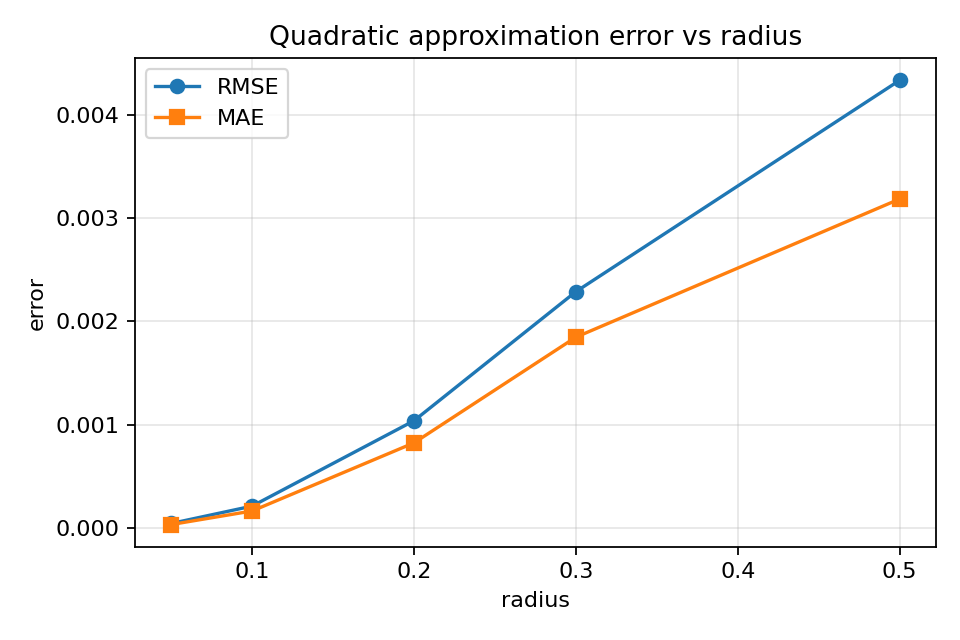
\includegraphics[width=0.72\textwidth]{figures/error_vs_radius.png}
    \caption{Error vs radius (linear scale).}
    \label{fig:error_vs_radius}
\end{figure}

\begin{figure}[H]
    \centering
    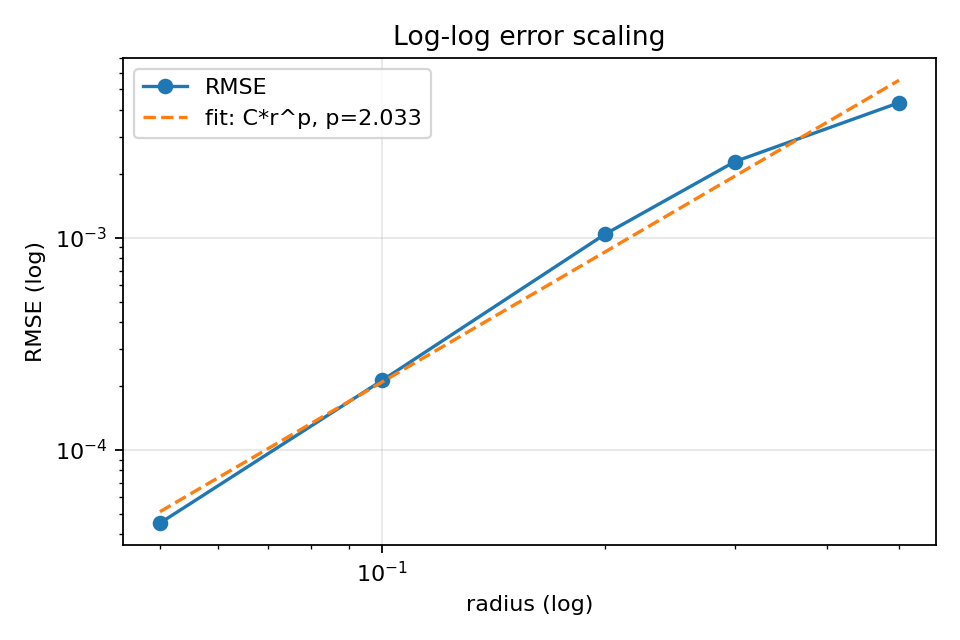
\includegraphics[width=0.72\textwidth]{figures/error_vs_radius_loglog.png}
    \caption{Error vs radius (log-log) и оценка показателя степени $p$.}
    \label{fig:error_vs_radius_loglog}
\end{figure}

\subsection{Training dynamics: flat vs sharp}

Для анализа динамики требуются checkpoint'ы ранних эпох. В текущем наборе артефактов присутствует только финальный checkpoint:
\begin{itemize}
    \item early (`epoch1`) --- TODO, отсутствует;
    \item middle (`epoch5`) --- TODO, отсутствует;
    \item final (`model1_final.pth`) --- доступен.
\end{itemize}

Для future-run в код обучения добавлена поддержка автосохранения checkpoint'ов `epoch1` и `epoch5`.

\begin{table}[H]
\centering
\begin{tabular}{lcccc}
\toprule
Checkpoint & $\lambda_{min}$ & $\lambda_{max}$ & Condition number & Sharpness \\
\midrule
final & 1.000e-06 & 1.000e-06 & 1.0 & 1.777e-03 \\
\bottomrule
\end{tabular}
\caption{Оценки кривизны и sharpness для доступного checkpoint.}
\label{tab:training_dynamics}
\end{table}

\begin{figure}[H]
    \centering
    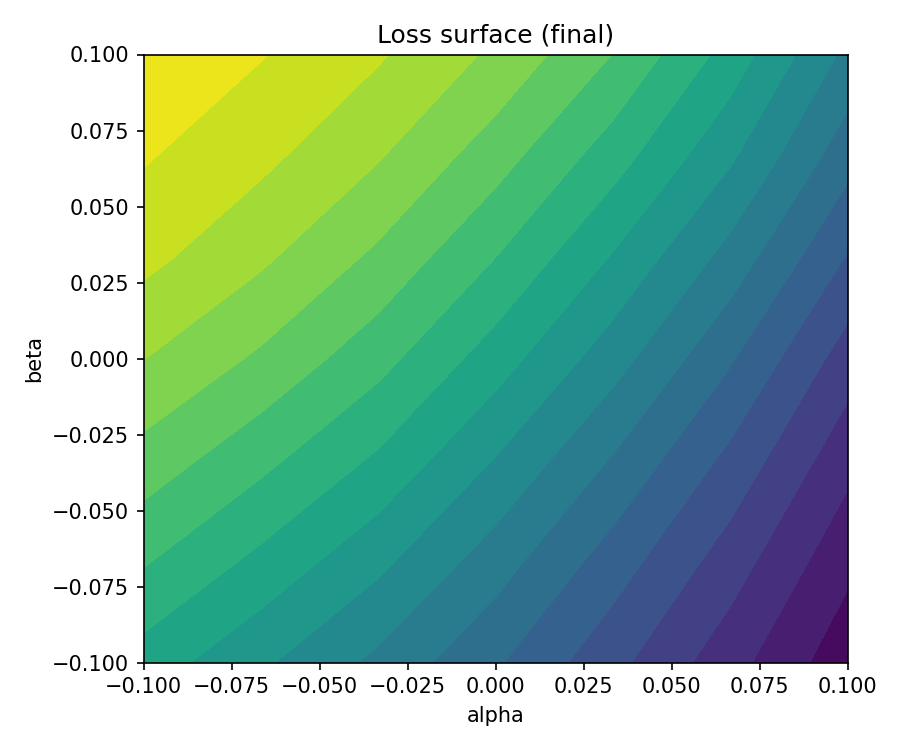
\includegraphics[width=0.72\textwidth]{figures/loss_surface_epoch_final.png}
    \caption{Loss surface для финального checkpoint.}
    \label{fig:loss_surface_final}
\end{figure}
